\section{Evaluation}
\label{sec-evaluation}

We evaluate PocketParker in three ways. First, we conducted a controlled
experiment to determine the correct parameter settings for our parking event
detector. Second, we have implemented a parking lot simulator, which allows
us to experiment with various kinds of lots as well as vary the monitored
fraction and other parameters. Finally, we performed a small-scale deployment
of PocketParker on our campus and use it to monitor three lots. Camera
monitoring was used to ground truth the predictions from our deployment
dataset. All three components of our evaluation together confirm that
PocketParker is efficiency and accurate.

\subsection{Detector Experiment}

\begin{figure}
\centering
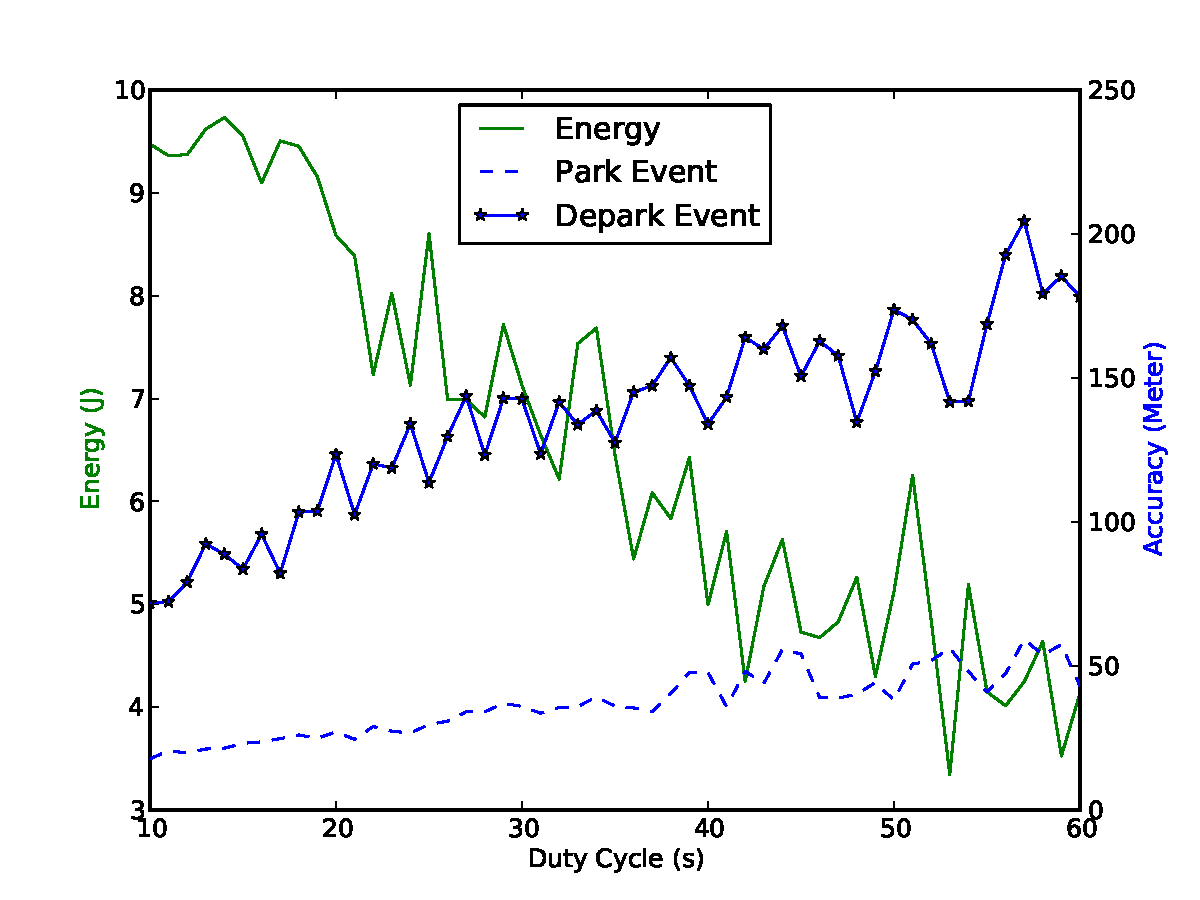
\includegraphics[width=3.325in]{./figures/Energy_accuracy.pdf}

\caption{\textbf{Power usage vs. detector accuracy.} Energy usage by
PocketParker is low at all duty cycles, so we chose an aggresive duty cycle
in order to improve detection accuracy.}

\label{fig-energy}
\end{figure}

\newcolumntype{b}{>{\hsize=1.4\hsize}X}
\newcolumntype{s}{>{\hsize=.6\hsize}X}
\begin{table}[t]
{\small
\begin{threeparttable}
\begin{tabularx}{\columnwidth}{b s b s}
  {{\textbf{Carry Location}}} & {{\textbf{Count}}} &
  {{\textbf{Car Location}}} &
  {{\textbf{Count}}} \\
 \hline
In hand & 18 & Cup holder & 16 \\
Side bag & 10 & Car seat  & 9 \\
Back pack & 10 & Side bag & 10 \\
In hand talking & 7 & Back pack & 9 \\
Front pocket & 14 & Front pocket & 14 \\
Jacket pocket & 14 & Jacket pocket & 14 \\
Back pocket & 7 & Back pocket & 14 \\
\end{tabularx}
\end{threeparttable}
\caption{\textbf{Carry and car location for detector experiment.}
Eight participants generated 80 runs, carrying and placing the
phone in their car in many ways.}
\label{table-experiment}
}
\vspace*{-0.1in}
\end{table}


To determine the right parameter settings for our transition detector, we
conducted a controlled experiment. During this experiment, accelerometer and
GPS data was collected continuously and store on each device, and
participants were asked to manually label each transition into and out of the
car. Afterwards, data was fed into Python-based simulator implementing the
same algorithm used by the PocketParker application, allowing us measure
accuracy and energy consumption as function of the detector duty cycle.

Eight volunteers participated, including seven men and one woman, seven of
whom were right-handed and one of whom was left-handed. Each was asked to
conduct the same experiment 10 times: carrying the instrumented phone, walk
out to their car, label departure, drive around briefly, park, label arrival,
and walk back inside. Since the way the phone is carried while walking and
placed in the car while driving affects the accelerometer readings, care was
taken to generate a good mix of carry and car location styles.
Table~\ref{table-experiment} shows the breakdown. The experiment permitted us
to obtain sensing data from a cross section of people posessed of varying
body morphologies and different habits of driving cars and handling mobile
devices. Participation in the experiment took roughly one hour and pizza was
provided.

Figure~\ref{fig-energy} displays the tradeoff between energy usage and
detection accuracy as a function of the PocketParker duty cycle. Here we
combine an active period of 5~s with a inactive period of variable length,
between 5~and~55~s, for an overall duty cycle between 0.5 and 0.06. Our
simulator uses energy numbers used by the Android Fuel Guage application
along with the acceloremeter duty cycles and number of GPS locations
requested including false positives to estimate average power consumption.
This graph measures the accuracy of detected events in terms of distance from
the actual location of the event labelled by the participant

As we expect, longer duty cycles consume less energy but produce longer
detection latencies which translate into higher distances from the event
location. Note also that the departure events have higher location error than
the parking events, simply because after departing users are driving and
therefore traveling more rapidly. Overall power usage by PocketParker is low,
under 10~mW at all duty cycles. Because PocketParker's ability to map parking
events into lots is affected by the detection distance accuracy, we chose a
relatively-aggresive total period of 15~s for a $\frac{1}{3}$ duty cycle.
This allows PocketParker to determine location to within 25~m for parking
events and 80~m for departures. Power consumption at this duty cycle is 8~mW,
representing 4.2\% of a the capacity of a 1500~mAh battery discharged over
24~hours if used continuously.

\subsection{Simulation Results}
\label{subsec-simulator}

To experiment with PocketParker in a more controlled setting, we implemented
a parking lot simulator in Python. Our simulator allows us to simulate any
number of parking lots associated with any number of points of interest with
varying desirability levels. For simplicity during our evaluation, we
simulate two lots 1~and~2 with lot~1 filling before lot~2, although lot
choice by simulated drivers is probabilistic. Particularly for evaluating our
monitored fraction estimation we are interested in lots that fill and empty
in various ways. We use five types of lots described by
Figure~\ref{fig-lotsdescription}:

\begin{itemize}

\item \textbf{Fast Fill} and \textbf{Slow Fill} fill once per day quickly or
slowly, like a lot associated with a place of work.

\item \textbf{High Churn} starts with lot~1 full and experiences continuously
high arrival and departures rates, like an airport parking lot.

\item \textbf{Low Churn} represents underutilized lots that never completely
fill, with lot~2 almost completely unused.

\item \textbf{Multiple Fill} represents a lot that rapidly fills and empties
repeatedly during each day, perhaps like a campus lot or movie theater.

\end{itemize}

\begin{figure*}
\centering
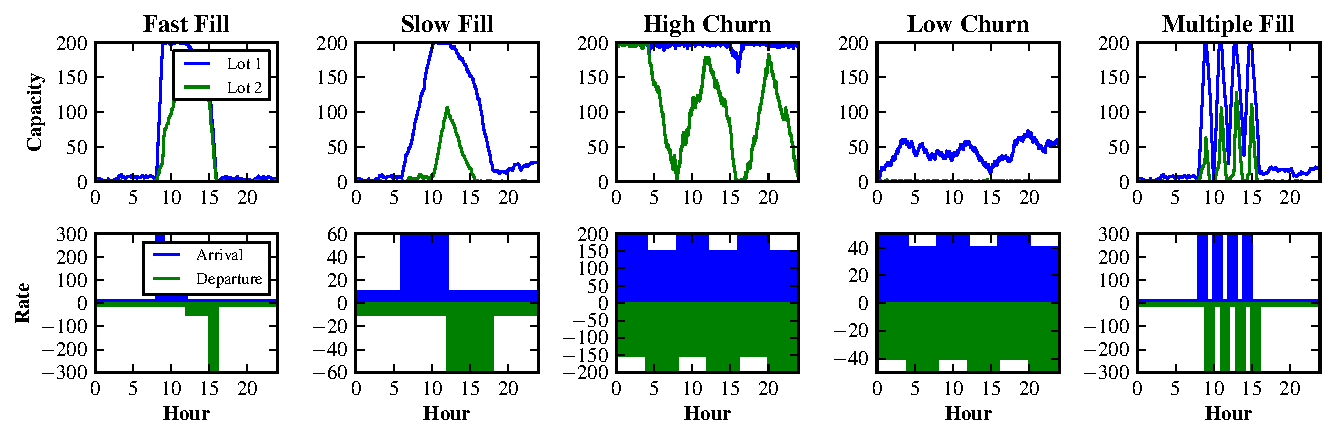
\includegraphics[width=\textwidth]{./simulator/figures/lots.pdf}

\caption{\textbf{Description of each type of lot simulated.} Five different
lots with different behaviors were used during simulations.}

\label{fig-lotsdescription}
\end{figure*}

\begin{figure*}
\centering
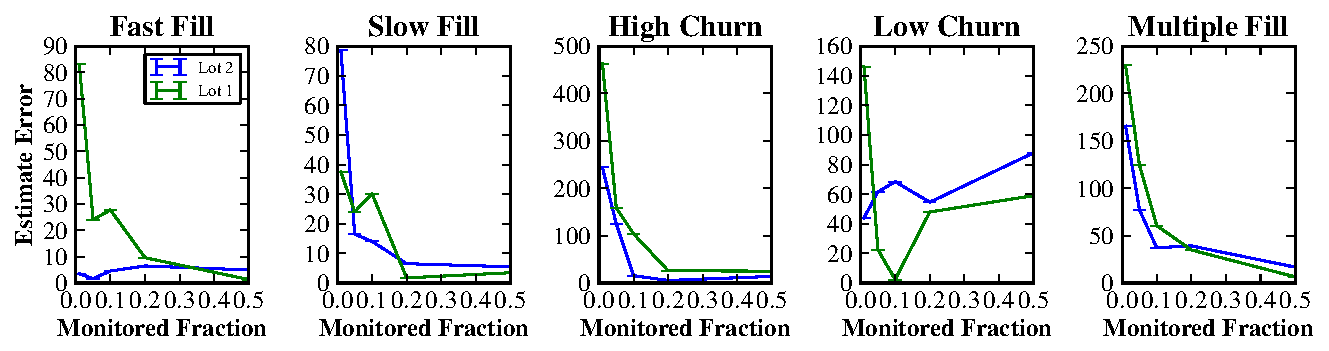
\includegraphics[width=\textwidth]{./simulator/figures/capacity_experiment.pdf}

\caption{\textbf{Errors in capacity estimation.} \XXXnote{GWA: TODO.}}

\label{fig-capacityerrors}
\end{figure*}

\begin{figure}
\centering
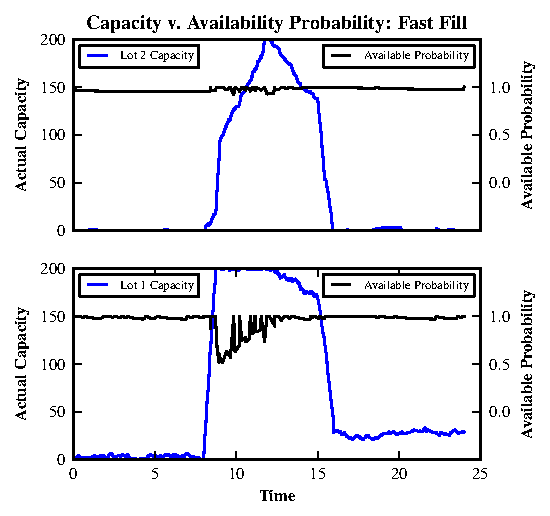
\includegraphics[width=3.325in]{./simulator/figures/tracking_fastfill.pdf}

\caption{\textbf{Availability probabilities tracking lot capacity.} \XXXnote{GWA: TODO.}}

\label{fig-trackingexample}
\end{figure}


\subsection{Deployment}

Finally, to establish the accuracy of PocketParker we performed a small-scale
deployment on campus. Five participants installed our PocketParker
application and generated 372 events over ten days---202 arrivals and 170
departures. Of those events, 127 occurred near campus including false
positives, and 56 were mapped into the three campus lots monitored by
PocketParker. One of the participants lives quite close to campus, and many
of the parking transitions that occurred at their house were included in the
127~events near campus. The deployment period included several days when
participants did not come to campus, and most parking events were generated
by three participants who came to campus daily. Figure~\ref{fig-events} shows
all of the events that occurred in the three lots we monitored. Our computer
science department is labeled as the point of interest.

Of the participants that installed PocketParker, none complained of excessive
energy usage or battery life problems. While the PocketParker interface
displays the last sensed state, no interaction with the application was
required or recorded.

\begin{figure*}
\centering
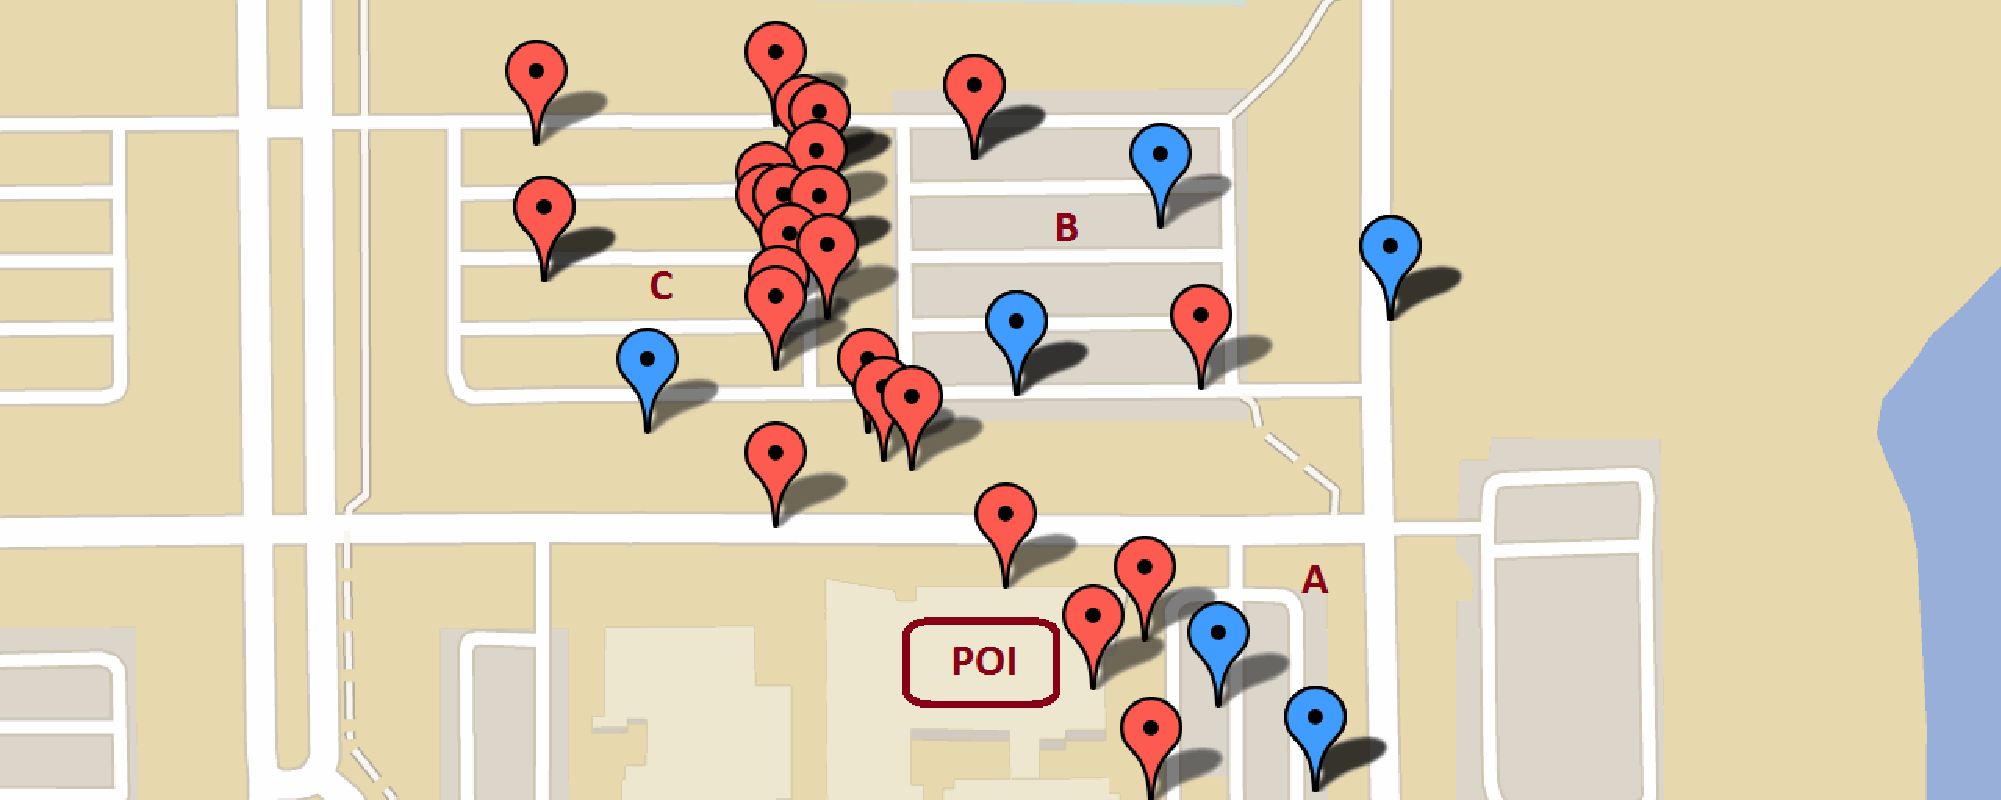
\includegraphics[width=\textwidth,height=2in]{./figures/detectedEventsOnMap.pdf}

\caption{\textbf{Map showing all events detected by PocketParker during our
ten-day deployment.} 56~events are shown in three monitored lots.}

\label{fig-events}
\end{figure*}

\begin{figure}
\centering
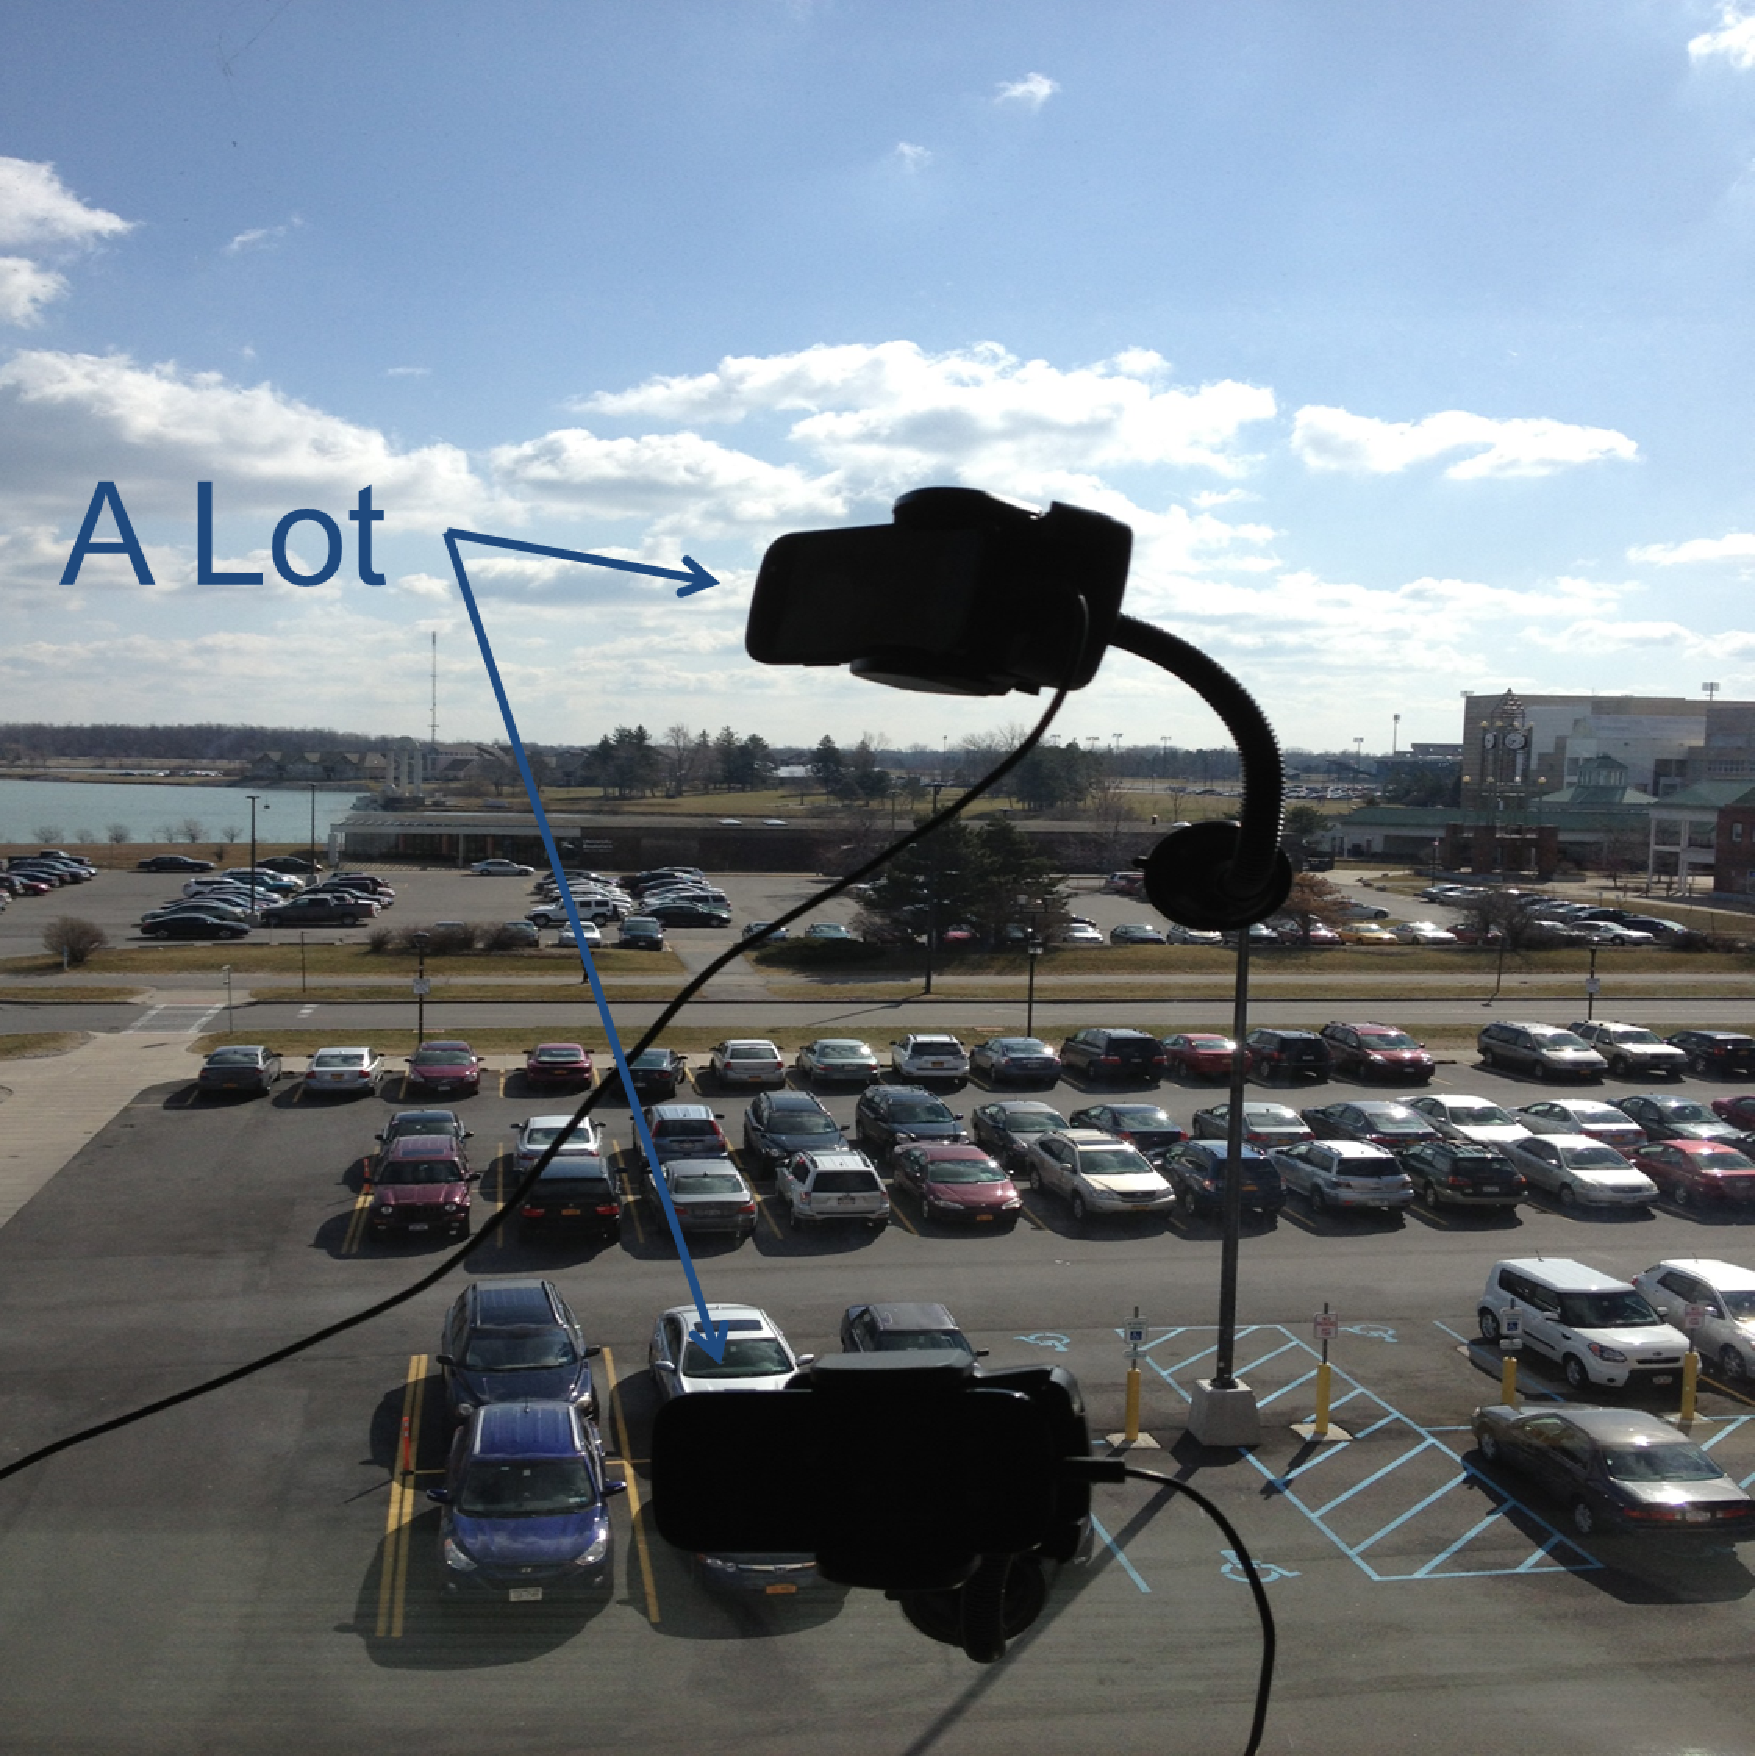
\includegraphics[width=3.0in]{./figures/Camera_setting.pdf}

\caption{\textbf{Monitoring cameras.} A view of one of the monitored parking
lots is shown.}

\label{fig-camera}
\end{figure}
